\documentclass[resume]{subfiles}



\begin{document}
\section{Espaces d'états}
\begin{figure}[H]
\centering
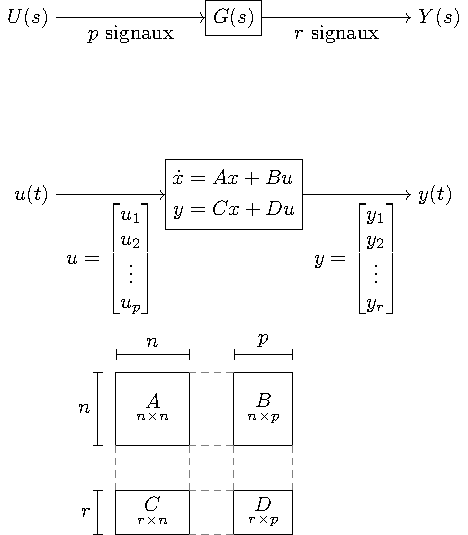
\includegraphics[scale=1,page=1]{drwg_0.pdf}
\end{figure}
\subsection{Choix des variables d'état}
Les variables d'état sont les variables qui ont leurs dérivée dans les équations.
\begin{itemize}
\item Condensateur : tension
\item Bobine : courant
\end{itemize}

\subsection{Forme modale}
Matrice $T$ construite à partir des vecteurs propres de $A$
$$T=\begin{bmatrix}
\\
\vec{v}_1 & \vec{v}_2 & \cdots\\
\\
\end{bmatrix}$$
$$\boxed{\begin{split}
\tilde{A} &= T^{-1}AT &\qquad \tilde{B}&=T^{-1}B\\
\tilde{C} &= CT&\qquad \tilde{D}&=D\end{split}}$$
\subsection{$A,B,C,D \longrightarrow G$}
$$G(s)=C(sI-A)^{-1}B+D$$
$$G(z)=C_n(zI-A_n)^{-1}B_n+D_n$$
\subsubsection{Gain haute fréquence}
$$\lim_{s\to\infty}G(s)=D$$
\subsubsection{Gain basse fréquence (gain statique)}
Analogique : $$G(s=0)=-CA^{-1}B+D$$
Numérique  : $$G(z=1)=-C(I-A)^{-1}B+D$$

\subsection{$G\longrightarrow A,B,C,D$}
On utilise la forme commandable
$$G(s)=\frac{b_2s^2+b_1s+b_0}{s^3+a_2s^2+a_1s+a_0}$$
$$\boxed{\begin{split}
A&=\begin{bmatrix}0 & 1 & 0\\0 & 0 &1\\-a_0 & -a_1 & -a_2\end{bmatrix} &
B&= \begin{bmatrix}
0\\0\\1
\end{bmatrix}\\
C&=\begin{bmatrix}b_0 & b_1 & b_2\end{bmatrix} & D&=0\end{split}}$$
\subsection{$G(s) / G(z) \longleftrightarrow A,B,C,D$}
\begin{figure}[H]
\centering
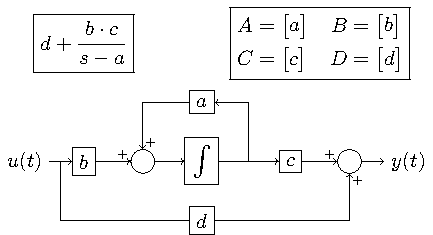
\includegraphics[scale=1,page=1]{drwg_1.pdf}\\
\includegraphics[scale=1,page=2]{drwg_1.pdf}
\end{figure}

\subsection{Conversion analogique vers numérique}
$$A_d = e^{A_a\cdot h}$$
$$B_d = \int_0^h e^{A_a\cdot\tau}B_a d\tau$$
$$C_d = C_a$$
$$D_d = D_a$$

\subsection{Mise en cascade}
\begin{figure}[H]
\centering
\includegraphics[scale=1,page=2]{drwg_0.pdf}
\end{figure}
$$S_{tot}=S_2(s)\cdot S_1(s)\qquad\text{ordre important}$$
$$A_{tot}=\begin{bmatrix}
A_1 & 0\\
B_2C_1 & A_2
\end{bmatrix}\qquad B_{tot}=\begin{bmatrix}
B_1\\B_2D_1
\end{bmatrix}$$
$$C_{tot}=\begin{bmatrix}
D_2C_1 & C_2
\end{bmatrix}\qquad D_{tot}=D_2D_1$$
\subsection{Mise en parallèle}
\begin{figure}[H]
\centering
\includegraphics[scale=1,page=3]{drwg_0.pdf}
\end{figure}
$$S_{tot}(s)=S_1(s)+S_2(s)$$
$$A_{tot}=\begin{bmatrix}
A_1 & 0\\0 & A_2
\end{bmatrix}\qquad B_{tot}=\begin{bmatrix}
B_1\\B_2
\end{bmatrix}$$
$$C_{tot}=\begin{bmatrix}
C_1 & C_2
\end{bmatrix}\qquad D_{tot}=D_1+D_2$$
\subsubsection{Mise en contre-réaction 1}
\begin{figure}[H]
\centering
\includegraphics[scale=1,page=4]{drwg_0.pdf}
\end{figure}
$$A_{tot}=\begin{bmatrix} A_1 - B_1D_2(I-D_1D_2)^{-1}C_1 & -B_1(C_2-D_2D_1C_2)\\B_2(I-D_1D_2)^{-1}C_1 & A_2-B_2(I-D_1D_2)^{-1}D_1C_2\end{bmatrix}\qquad B_{tot}=\begin{bmatrix}B_1-B_1D_2ND_1\\B_2ND_1\end{bmatrix}$$

$$C_{tot}=\begin{bmatrix}(I-D_1D_2)^{-1}C_1 & -(I-D_1D_2)^{-1}D_1C_2\end{bmatrix}\qquad D_{tot}=(I-D_1D_2)^{-1}D_1$$ 

\subsubsection{Mise en contre-réaction 2}
\begin{figure}[H]
\centering
\includegraphics[scale=1,page=5]{drwg_0.pdf}
\end{figure}
$$S_{tot}(s)=\left(I+S_1(s)S_2(s)\right)^{-1}S_1(s)$$
$$A_{tot}=\begin{bmatrix}A_1 & 0\\B_2C_1 & A_2\end{bmatrix}\qquad B_{tot}=\begin{bmatrix}B_1\\B_2D_1\end{bmatrix}$$
$$C_{tot}=\begin{bmatrix}
D_2 C_1 & C_2
\end{bmatrix}\qquad D_{tot}=D_1D_2$$
\subsection{Commandabilité}
$$\boxed{P_c=\begin{bmatrix}B & AB & \cdots & A^{n-1}B\end{bmatrix}}$$
Pour des systèmes monoentrée :
$$\det(P_c)\neq 0\longrightarrow \text{Commandable}$$
Pour des systèmes multi-entrées (généralisation) :
$$\text{rang}(P_c)==n\longrightarrow \text{Commandable}$$
Faire une permutation avec $T$ ne change pas la commandabilité du système. La nouvelle matrice $\tilde{P}_c$ est donnée par $T^{-1}P_c$
\subsection{Observabilité}
$$\boxed{P_0=\begin{bmatrix}C\\CA\\CA^2\\\vdots\\CA^{n-1}\end{bmatrix}}$$
$$\boxed{\text{rang}(P_0)=n\longrightarrow\text{Observable}}$$
En monosortie on peut utiliser $\det(P_0)\neq 0\longrightarrow \text{Observable}$
\subsection{Trajectoire}
\subsection{Système numérique}
Soit un système numérique avec les matrices
$$A_n\qquad B_n\qquad C_n\qquad D_n$$
Et la condition initiale $x_0$. On chercher à trouver les valeurs de $x[0],x[1],x[2],\cdots$
$$x[k]=\textcolor{OrangeRed}{A_n^kx[0]}+\textcolor{RoyalBlue}{A_n^{k-1}B_nu[0]+A_n^{k-2}B_nu[1]+\cdots +B_nu[k-1]}$$
On a la \textcolor{OrangeRed}{contribution de la condition initiale} et un \textcolor{RoyalBlue}{produit de convolution} $u[k]\ast g_x[k]$
\subsubsection{Réponse impulsionnelle}
Si on suppose que la condition initiale est nulle et qu'on excite le signal avec un dirac numérique, alors on a
$$\boxed{x[k]=A_n^{k-1}B_n}$$
\subsection{Système analogique}
Soit un système numérique avec les matrices
$$A_n\qquad B_n\qquad C_n\qquad D_n$$
Et la condition initiale $x_0$
$$\boxed{x(t)=\textcolor{OrangeRed}{e^{At}x_0}+\textcolor{RoyalBlue}{\int_{0}^{t}e^{A(t-\tau)}Bu(\tau)d\tau}}$$
\subsubsection{Exponentielle matricielle (ou matrice de transition)}
$$\boxed{e^{At}=I+At+\frac{(At)^2}{2!}+\frac{(At)^3}{3!}+\cdots}$$
Si $A$ est diagonale, on peut simplifier en écrivant
$$e^{At}=\begin{bmatrix}e^{a_{11}t} & 0 & 0\\0 & e^{a_{22}t} & 0\\0 & 0 & e^{a_{33}t}\end{bmatrix}$$
\paragraph{Calcul par diagonalisation}
Si $A$ est diagonalisable, alors
$$\boxed{e^{At}=Te^{\tilde{A}t}T^{-1}}$$
Ceci permet de simplifier les calculs en utilisant la propriété de l'exponentielle lorsque $\tilde{A}$ est diagonal

\subsection{Forme commandable}
\begin{figure}[H]
\centering
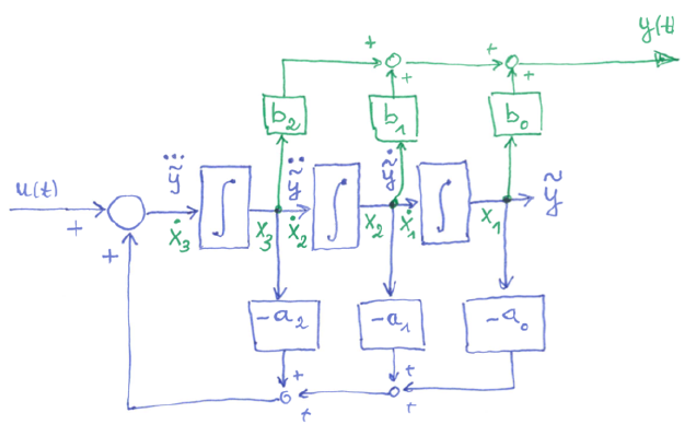
\includegraphics[width=\columnwidth]{img_0.png}
\end{figure}
On obtient donc finalement
$$\boxed{\begin{split}
A&= \begin{bmatrix}0 & 1 & 0\\0 & 0 & 1\\-a_0 & -a_1 & -a_2\end{bmatrix} & B&=\begin{bmatrix}0\\0\\1\end{bmatrix}\\
C&=\begin{bmatrix}b_0 & b_1 & b_2\end{bmatrix} & D&=0
\end{split}}$$
Voir \ref{sec_eq_diff}

\subsection{Modèle échantillonné}
$$\boxed{H(z)=\frac{z-1}{z}Z\left(\mathcal{L}^{-1}\left(\frac{G_a(s)}{s}\right)\Big|_{t=kh}\right)}$$
\subsubsection{Représentation dans l'espace d'état}
$$\boxed{\begin{split}
A_n&=e^{Ah} & B_n&=\int_{0}^{h}e^{A\tau}Bd\tau\\
C_d&=C & D_n &= D
\end{split}}$$



\subsection{Action intégrale sur la commande}
\begin{figure}[H]
\centering
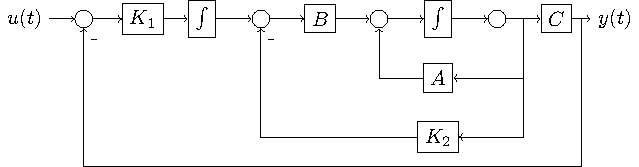
\includegraphics[width=\columnwidth]{drwg_2.pdf}
\end{figure}
$$\hat{A}=\begin{bmatrix}0 & C\\0 & A\end{bmatrix}\qquad \hat{B}=\begin{bmatrix}0\\B\end{bmatrix}$$


\subsection{Placement de pôles}
Il faut que le polynôme caractéristique de la boucle fermée (par exemple $sI-A_{bf}=sI-(A-BK)$) corresponde aux pôles que l'ont souhaite
$$\det(sI-A_{bf})=(s-p_1)(s-p_2)\cdots(s-p_n)$$

\subsection{Retour d'état}
$$A_{bf}=A-BK$$
\end{document}